\chapter{Mouse Behaviour in Complex VR Tasks}
\label{chapterlabel3}

\section{Can Mouse Learn Visually Complex Navigation Task?}
 Many recent studies in mouse VR navigation tasks use tall and large visual landmarks which can be seen and distinguished from far away with floor patterns as only background. In the experiment design I use, it presents the challenge to the mouse that it needs to differentiate sets of identical landmarks in grayscale and the well-controlled white noise gray background. Compared to primates, cats, birds, mice have low acuity vision. One may argue that mouse cannot differentiate such detailed visual landmarks in a VR setting to form clear representations of the space. In Saleem et al. 2018, they've trained the mice to actively lick for a reward associated to one of the identical plaid landmarks spaced at 20cm in a 100 cm corridor. Here in one of the environment, I use a familiar set of landmarks but with an additional cue landmark at the start with extension of extra 40 cm. Further to that, the VR corridor is constrained to only show 21cm ahead of the mouse rather than the full view ahead. This method prevents the mouse knowing what landmarks are ahead until it passes the current landmark and it is different from the conventional VR task particularly in studies on hippocampus and entorhinal cortices. Therefore, it can be perceptually more challenging to distinguish one visual landmark and 2 sets of identical visual landmarks in 100 cm space. In addition, in the recording period, there would be an extra environment introduced to the animal and the novel environment contains one of the same set of landmarks, that is, the plaids, and the mouse is required to distinguish the two environments are different. In this chapter, I will show mice can learn visually complex navigation tasks.

\section{Methods}

\section{Mice }

\begin{figure}
    \centering
    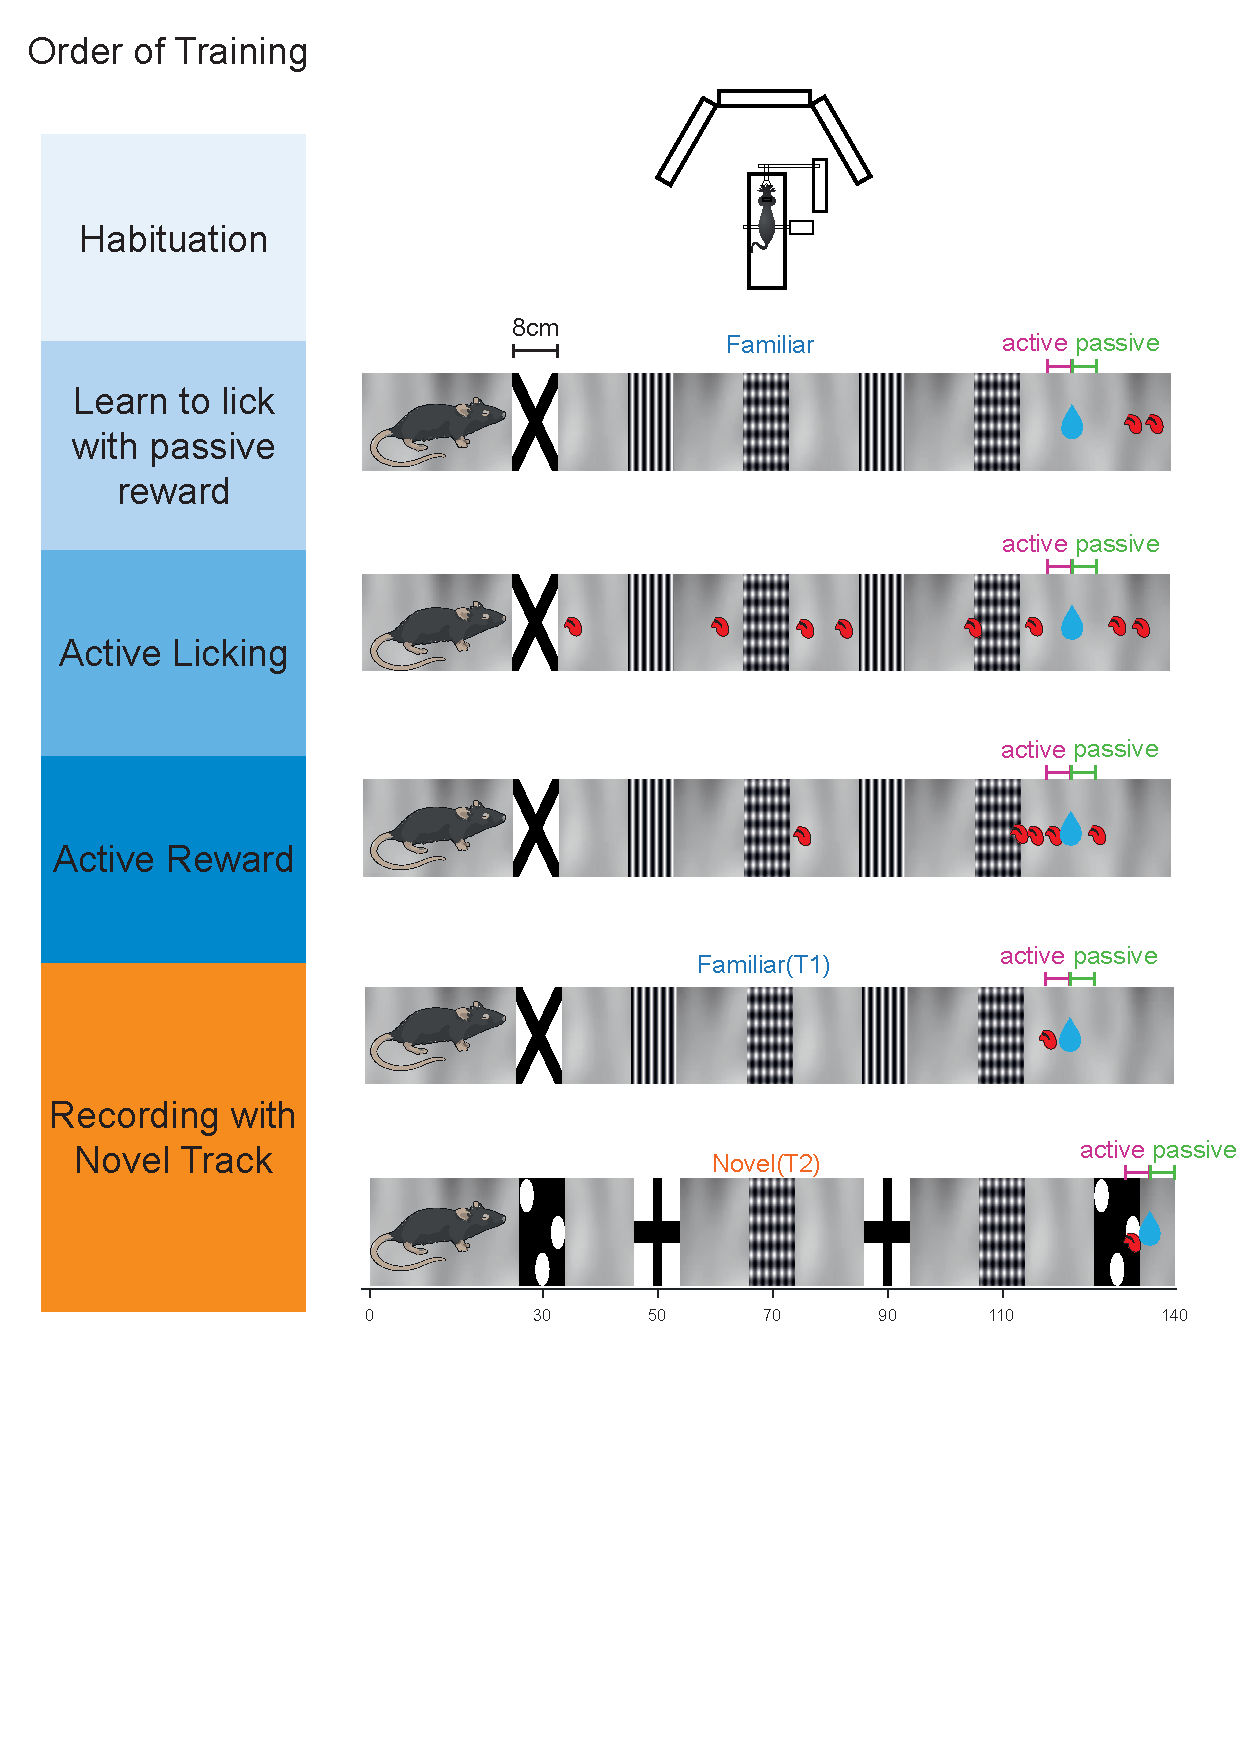
\includegraphics[width=1\linewidth]{figures//Chapter 3 Behaviour//Thesis Figures//figure_PDFs/fig1_behaviour_training.pdf}
    \caption{An illustration of stages of training from habituation to recordings. The illustration gives examples of licking behaviour over stages of training. In early stage, the mouse can only lick after a passive reward is given. After habituation to the reward and licking, the mouse can lick actively everywhere in the VR. Once learned, the active licking is more likely to be around reward zone. Once the mouse is ready, it undergoes craniotomy surgery and the ephys recordings start with the introduction of novel VR environment.}
    \label{fig:placeholder}
\end{figure}


